\documentclass{article}

\usepackage{../../common}

\graphicspath{
  {../../../media/images/}
}
\addbibresource{../../references.bib}

\title{Počtové výkony s prirodzenými číslami}
\begin{document}

\maketitle

\section{Porovnávanie a usporiadanie prirodzených čísel}

Porovnávanie prirodzených čísel znamená určiť, ktoré číslo je väčšie, menšie alebo či sú obe čísla rovnaké. V desiatkovej číselnej sústave je desať rôznych číslic v poradí od najmenšej po najväčšiu: \(0\), \(1\), \(2\), \(3\), \(4\), \(5\), \(6\), \(7\), \(8\) a \(9\). Každá číslica vyjadruje určitú hodnotu. Väčšie čísla sú tvorené kombináciou týchto desiatich číslic.

Každé číslo dokážeme usporiadať tak, aby výsledná postupnosť čísel bola zoradená podľa veľkosti. Usporiadanie znamená vytvorenie určitej postupnosti. Usporiadaním prirodzených čísel vytvoríme postupnosť čísel \(0\), \(1\), \(2\), \(3\), \(4\), \(5\), \(6\), \(7\), \(8\), \(9\), \(10\), \(11\), \(12\)\dots atď. Susedné čísla sa líšia o hodnotu jeden. Graficky by sa táto postupnosť dala znázorniť ako číselná os.

\begin{center}
  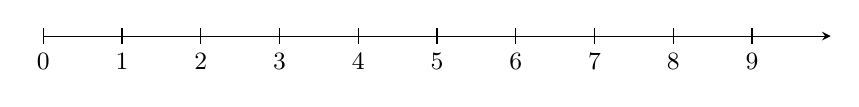
\begin{tikzpicture}[>=stealth]
    \draw[->] (0,0) -- (10,0);
    \foreach \x in {0,1,...,9}
    {
      \draw (\x,0.1) -- (\x,-0.1);
      \node[below] at (\x,-0.1) {\small $\x$};
    }
  \end{tikzpicture}
\end{center}

Usporiadania môžu byť dvojakého typu: od najmenšieho čísla po najväčšie číslo, nazývané ako vzostupné, a od najväčšieho čísla po najmenšie číslo, nazývané ako zostupné. Pre potreby porovnávania sa používa vzostupné usporiadanie čísel.

Vzostupné usporiadanie prirodzených čísel umožňuje zaviesť vzťahy, pomocou ktorých porovnávame čísla na základe ich veľkosti. Pre dve prirodzené čísla \(a\) a \(b\) môžeme zaviesť nasledovné vzťahy:
\begin{itemize}
  \item Číslo \(a\) je väčšie ako číslo \(b\), ak sa na číselnej osi nachádza napravo od čísla \(b\).
  \item Číslo \(a\) je menšie ako číslo \(b\), ak sa na číselnej osi nachádza naľavo od čísla \(b\).
  \item Číslo \(a\) sa rovná číslu \(b\), ak sa na číselnej osi nachádzajú v tom istom bode.
\end{itemize}
Zhrnutím do jednej vety môžeme povedať, že z dvoch prirodzených čísel je väčšie to, ktorého obraz na číselnej osi je ďalej od nuly. Na základe tohto môžeme definovať šesť typov porovnávania čísel: väčší ako, menší ako, rovná sa, väčší alebo rovná sa, menší alebo rovná sa a nerovná sa. V tabuľke sú ku každému porovnávaniu priradené aj symbolické zápisy.

\begin{table}[H]
  \centering
  \renewcommand{\arraystretch}{1.3}
  \begin{tabular}{|l|c|}
    \hline
    \multicolumn{1}{|c|}{Porovnávanie} &
    \multicolumn{1}{c|}{Znak} \\
    \hline
    Väčší ako & \(>\) \\
    Menší ako & \(<\) \\
    Rovná sa & \(=\) \\
    Väčší alebo rovná sa & \(\geq\) \\
    Menší alebo rovná sa & \(\leq\) \\
    Nerovná sa & \(\neq\) \\
    \hline
  \end{tabular}
  \caption{Prehľad porovnávaní a ich symbolický zápis.}
\end{table}

Pre dve prirodzené čísla \(a\) a \(b\), kde:
\begin{itemize}
  \item číslo \(a\) je väčšie ako číslo \(b\), platí \(a > b\),
  \item číslo \(a\) je menšie ako číslo \(b\), platí \(a < b\),
  \item číslo \(a\) sa rovná číslu \(b\), platí \(a = b\),
  \item číslo \(a\) je väčšie alebo sa rovná číslu \(b\), platí \(a \geq b\),
  \item číslo \(a\) je menšie alebo sa rovná číslu \(b\), platí \(a \leq b\),
  \item číslo \(a\) sa nerovná číslu \(b\), platí \(a \neq b\).
\end{itemize}
Porovnávať dve ľubovoľné prirodzené čísla môžeme týmto postupom v tomto poradí:
\begin{enumerate}[label=\arabic*)]
  \item Číslo s väčším počtom číslic je väčšie.
  \item Ak majú čísla rovnaký počet číslic, porovnávame ich číslice zľava doprava. Číslo je väčšie, ak má väčšiu číslicu v prvej nezhode.
  \item Ak sú všetky číslice rovnaké, čísla sú rovnaké.
\end{enumerate}

\section{Zaokrúhľovanie prirodzených čísel}

Zaokrúhľovanie je postup, kde nahrádzame číslo iným menej presným číslom, ktoré je jednoduchšie na čítanie, zapisovanie alebo počítanie. Používa sa vtedy, keď nepotrebujeme pracovať s úplne presnou hodnotu. Zaokrúhľovanie používame pri bežných odhadoch (napríklad koľko približne stojí nákup), pri meraní (dĺžka, hmotnosť, teplota), v štatistikách alebo pri rýchlych výpočtoch. Pri zaokrúhľovaní sa snažíme zmeniť číslo čo najmenej, aby sa výsledok čo najpresnejšie približoval k reálnej hodnote.

Pri zaokrúhľovaní nahradíme zaokrúhľované číslo jemu blízkym číslom. Zaokrúhľujeme najčastejšie na určitý číselný rád. Zaokrúhľovaním na určitý čiselný rád musíme dostať číslo, ktoré je násobkom tohto číselného rádu. Pri zaokrúhľovaní čísla na desiatky bude výsledok násobkom desiatky, pri zaokrúhľovaní čísla na stovky bude výsledok násobkom stovky atď. Na aký násobok číselného rádu zaokrúhľujeme číslo má vplyv číslica nižšieho rádu, ktorá sa nazýva rozhodujúca číslica. Pri zaokrúhľovaní na desiatky je rozhodujúca číslica rádu jednotiek, pri zaokrúhľovaní na stovky je rozhodujúca číslica rádu desiatok atď. Výsledkom zaokrúhľovania je číslo, v ktorom sú rozhodujúca číslica a všetky číslice nižších rádov nahradené nulami.

Podľa toho, či zaokrúhľujeme na menší alebo väčší násobok, rozlišujeme tri typy zaokrúhľovania čísel: zaokrúhľovanie nadol, zaokrúhľovanie nahor a aritmetické zaokrúhľovanie.
\begin{itemize}
  \item Pri zaokrúhľovaní nadol je výsledkom najbližšie prirodzené číslo, ktoré je menšie alebo sa rovná zaokrúhľovanému číslu.
  \item Pri zaokrúhľovaní nahor je výsledkom najbližšie prirodzené číslo, ktoré je väčšie alebo sa rovná zaokrúhľovanému číslu.
  \item Pri aritmetickom zaokrúhľovaní sa zaokrúhľuje buď nahor alebo nadol. Ak rozhodujúca číslica je \(0\), \(1\), \(2\), \(3\), \(4\), zaokrúhľujeme nadol. Ak rozhodujúca číslica je \(5\), \(6\), \(7\), \(8\), \(9\), zaokrúhľujeme nahor. Prívlastok aritmetické sa zvykne vynechávať, teda ak je v úlohe uvedené "zaokrúhlite", ide o aritmetické zaokrúhľovanie.
\end{itemize}



\section{Operácie s prirodzenými číslami}

Operácia je postup, podľa ktorého z jedného alebo viacerých matematických objektov (napríklad čísel) vytvoríme nový matematický objekt. Každá operácia má operandy a výsledok.

\subsection{Sčítanie prirodzených čísel}

Sčítanie je operácia, pri ktorej spájame dve alebo viac množstiev do jedného celku. Operáciu sčítania zapisujeme znakom \enquote{\(+\)}. Čísla, ktoré sčítavame, sa nazývajú sčítance a výsledok sčítania sa nazýva súčet.

V matematike sa sčítanie prirodzených čísel dá presne definovať pomocou pojmu nasledovník. Nasledovník prirodzeného čísla je číslo, ktoré vznikne pridaním jednotky k danému číslu. Každé prirodzené číslo má priradené číslo, ktoré nasleduje za ním. Prirodzené číslo \(0\) má nasledovníka číslo \(1\), prirodzené číslo \(1\) má nasledovníka číslo \(2\) atď. Takto vznikne postupnosť čísel \(0\), \(1\), \(2\), \(3\), \(4\), \(5\), \(6\), \(7\), \(8\), \(9\), \(10\), \(11\), \(12\)\dots Nasledovníka nejakého prirodzeného čísla \(a\) budeme označovať \(S(a)\). Nasledovníci niektorých prirodzených čísel sú:
\[
\begin{aligned}
  S(0) &= 1, \\
  S(1) &= 2, \\
  S(2) &= 3, \\
  S(3) &= 4, \\
  S(4) &= 5, \\
  S(5) &= 6, \\
  S(6) &= 7, \\
  S(7) &= 8, \\
  S(8) &= 9, \\
  S(9) &= 10.
\end{aligned}
\]
Sčítanie prirodzených čísel môžeme definovať pomocou dvoch základných pravidiel:
\[
\begin{aligned}
  \text{(1)}\quad a + 0 &= a \\
  \text{(2)}\quad a + 1 &= S(a)
\end{aligned}
\]
Pravidlo (1) hovorí, že ak k ľubovoľnému prirodzenému číslu \(a\) pripočítame nulu, hodnota čísla sa nezmení. Nula teda pri sčítaní neovplyvňuje výsledok. Pravidlo (2) vyjadruje vzťah medzi sčítaním a pojmom nasledovníka. Ak k číslu \(a\) pripočítame jednotku, dostaneme jeho nasledovníka. Zároveň platí aj opak, akékoľvek prirodzené číslo väčšie ako nula môžeme vyjadriť ako súčet predchodcu a jednotky. Tieto dve pravidlá nám umožňujú postupne definovať súčet ľubovoľných dvoch prirodzených čísel. Ak chceme vypočítať súčet čísel \(a\) a \(b\), môžeme číslo \(b\) chápať ako opakované pridávanie jednotky. Každá pripočítaná jednotka posunie číslo \(a\) k jeho ďalšiemu nasledovníkovi. Ako konkrétny príklad si môžeme zobrať čísla \(2\) a \(5\).
\[
\begin{aligned}
  &2 + 5, \\
  &2 + 4 + 1, \\
  &2 + 3 + 1 + 1, \\
  &2 + 2 + 1 + 1 + 1, \\
  &2 + 1 + 1 + 1 + 1 + 1, \\
  &3 + 1 + 1 + 1 + 1, \\
  &4 + 1 + 1 + 1, \\
  &5 + 1 + 1, \\
  &6 + 1, \\
  &7.
\end{aligned}
\]
Sčítanie teda môžeme chápať ako postupné vytváranie nasledovníkov: druhé číslo \(b\) určuje, koľkokrát máme od čísla \(a\) prejsť k jeho nasledovníkom. Výsledok sčítania dvoch prirodzených čísel \(a + b\) je číslo \(c\), ktoré dostaneme po prevedení čísla \(b\) na súčet jednotiek a postupným prevodom čísla \(a\) na nasledovníkov. Je to zdĺhavý postup sčítania dvoch čísel, a preto existujú efektívne algoritmy na sčítanie ľubovoľných prirodzených čísel. Pri sčítaní jednociferných čísel je časovo najvýhodnejšie zapamätať si základné spoje ščítania, ktoré sú ukázané v tabuľke.

\begin{table}[H]
\centering
\renewcommand{\arraystretch}{1.3}
\newcolumntype{C}{>{\centering\arraybackslash}m{1em}}
\begin{tabular}{C|CCCCCCCCCC}
\(+\) & 0 & 1 & 2 & 3 & 4 & 5 & 6 & 7 & 8 & 9 \\
\hline
0 & 0 & 1 & 2 & 3 & 4 & 5 & 6 & 7 & 8 & 9 \\
1 & 1 & 2 & 3 & 4 & 5 & 6 & 7 & 8 & 9 & 10 \\
2 & 2 & 3 & 4 & 5 & 6 & 7 & 8 & 9 & 10 & 11 \\
3 & 3 & 4 & 5 & 6 & 7 & 8 & 9 & 10 & 11 & 12 \\
4 & 4 & 5 & 6 & 7 & 8 & 9 & 10 & 11 & 12 & 13 \\
5 & 5 & 6 & 7 & 8 & 9 & 10 & 11 & 12 & 13 & 14 \\
6 & 6 & 7 & 8 & 9 & 10 & 11 & 12 & 13 & 14 & 15 \\
7 & 7 & 8 & 9 & 10 & 11 & 12 & 13 & 14 & 15 & 16 \\
8 & 8 & 9 & 10 & 11 & 12 & 13 & 14 & 15 & 16 & 17 \\
9 & 9 & 10 & 11 & 12 & 13 & 14 & 15 & 16 & 17 & 18 \\
\end{tabular}
\caption{Tabuľka súčtov čísel od 0 do 9.}
\end{table}

\subsection{Odčítanie prirodzených čísel}

\subsection{Násobenie prirodzených čísel}

\subsection{Delenie prirodzených čísel}

\end{document}